\appendix
\chapter{Fault-tolerant quantum computation}

\section{Fault-tolerant syndrome measurements}
\label{Ap:FT_syndrome_meas}
In the case of the stabilizer code, the syndrome measurements are done by simply measuring the stabilizer operators.
Several QEC gadgets have been proposed to implement the stabilizer measurement fault-tolerantly \cite{DiViShor,KnillNature,Steane97}.

{\it DiVincenzo-Shor's gadget---}
The first QEC gadget was proposed by David DiVincenzo and Peter Shor, who used cat states as ancillae for the syndrome measurement \cite{DiViShor}.
It is based on an indirect measurement of the observable $A$ with the eigenvalues $\pm 1$:
%
\begin{equation}
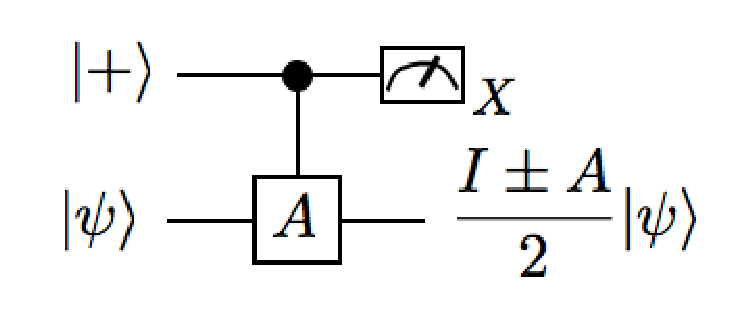
\includegraphics[width=70mm]{fig43.eps}
\label{eq:proj_meas}
\end{equation}
%
For example, the stabilizer $S_{1}$ of the seven-qubit code can be measured as the transversal $X$ measurements of the corresponding physical qubits in the code block:
%
\begin{equation}
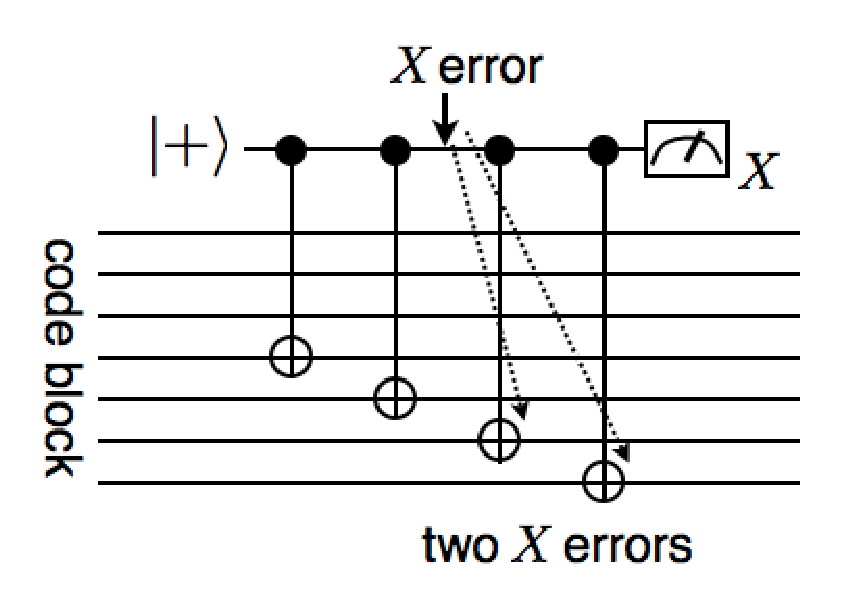
\includegraphics[width=70mm]{fig44.eps}
\end{equation}
%
Unfortunately, this measurement is not fault tolerant, because the errors in the CNOT gates [$A=X$ in Eq.\ (\ref{eq:proj_meas})] are spread by the following CNOT gates, as shown in the above circuit.
To make it fault-tolerant, a cat state $|{\rm cat} \rangle = ( | 000 \cdots 0\rangle + | 111 \cdots 1\rangle)/\sqrt{2}$ is used as an ancilla for the measurement as follows:
%
\begin{equation}
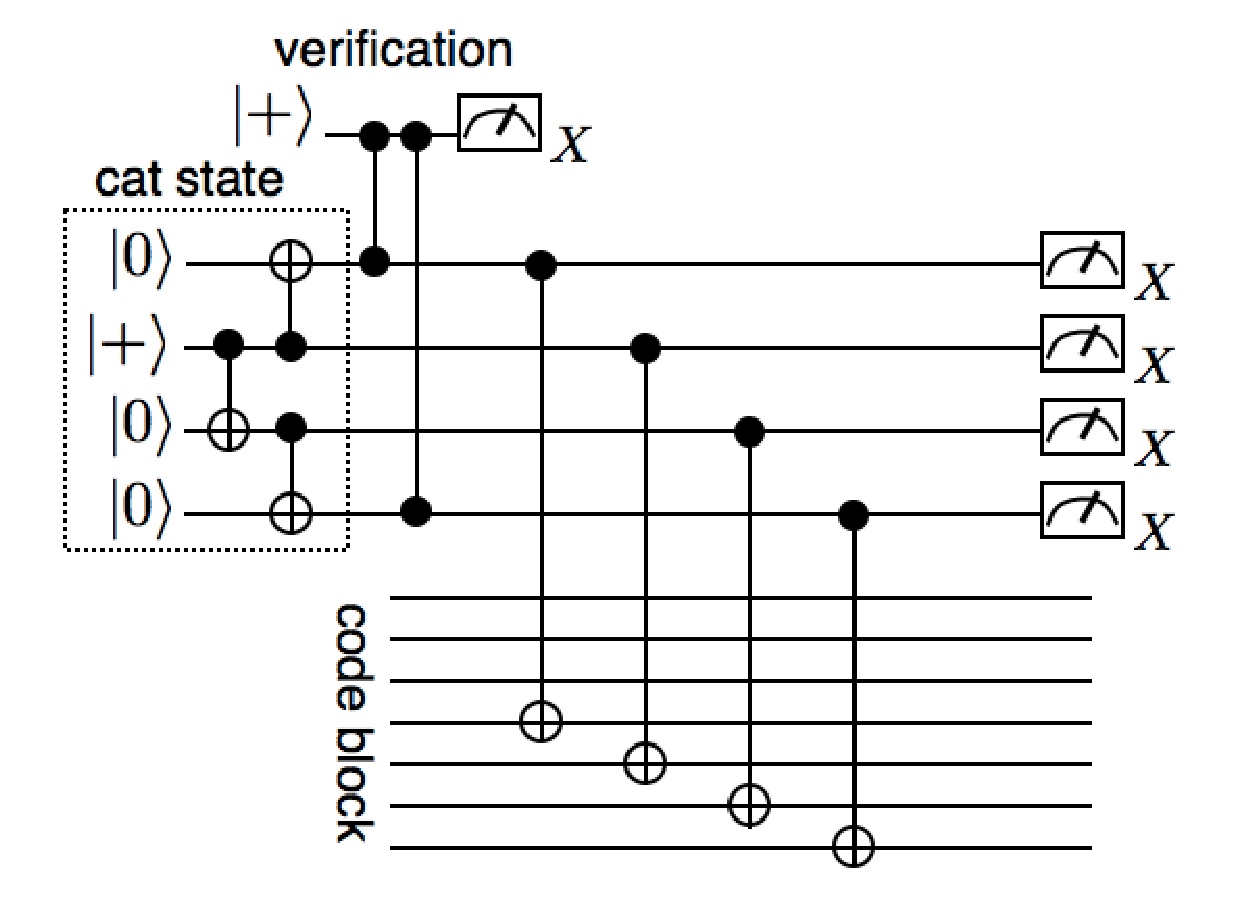
\includegraphics[width=90mm]{fig46.eps}
\end{equation}
%
where the cat state is verified before connecting with the code state.
Because the qubits in the code block interact with different ancilla qubits, this measurement does not spread the errors in the CNOT gates.
Similarly, other stabilizers $S_{2}, \cdots, S_{6}$ are measured fault-tolerantly to obtain the error syndrome.
Instead of the verification, one can perform a suitable recovery operation by postprocessing the ancilla state after its interaction with the code state \cite{DiVincenzo07}:
%
\begin{equation}
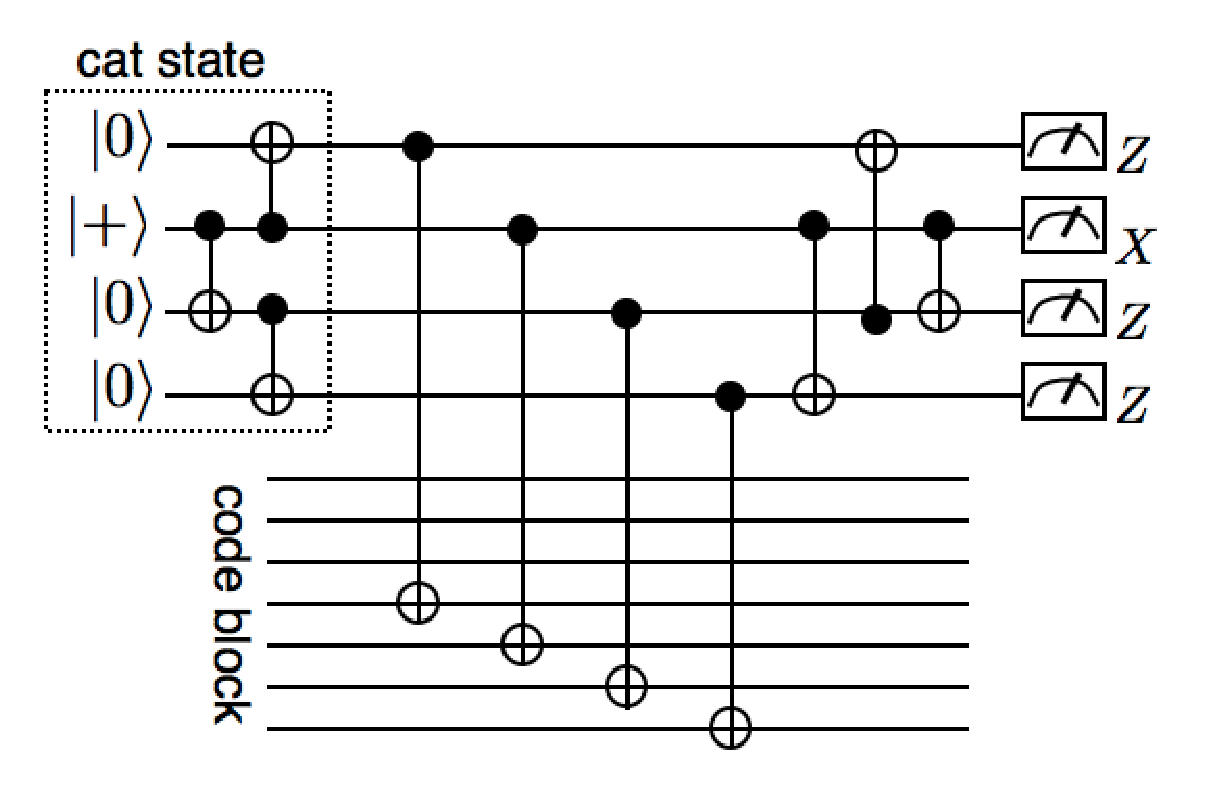
\includegraphics[width=90mm]{fig45.eps}
\end{equation}
%
The DiVincenzo-Shor's QEC gadget and its improved version both require a lot of physical gate operations, which results in deterioration of the performance.

{\it Steane's gadget---}
Subsequently, a relatively simple QEC gadget was proposed by Andrew Steane \cite{Steane97}, where encoded ancilla states are used to extract the syndrome with transversal operations.
In particular, for the case of the CSS code, the logical code states can be used as ancilla states.
The following circuit executes the $Z$ and $X$ error syndrome extractions by using the ancilla $ | 0_L \rangle $ states,
%
\begin{equation}
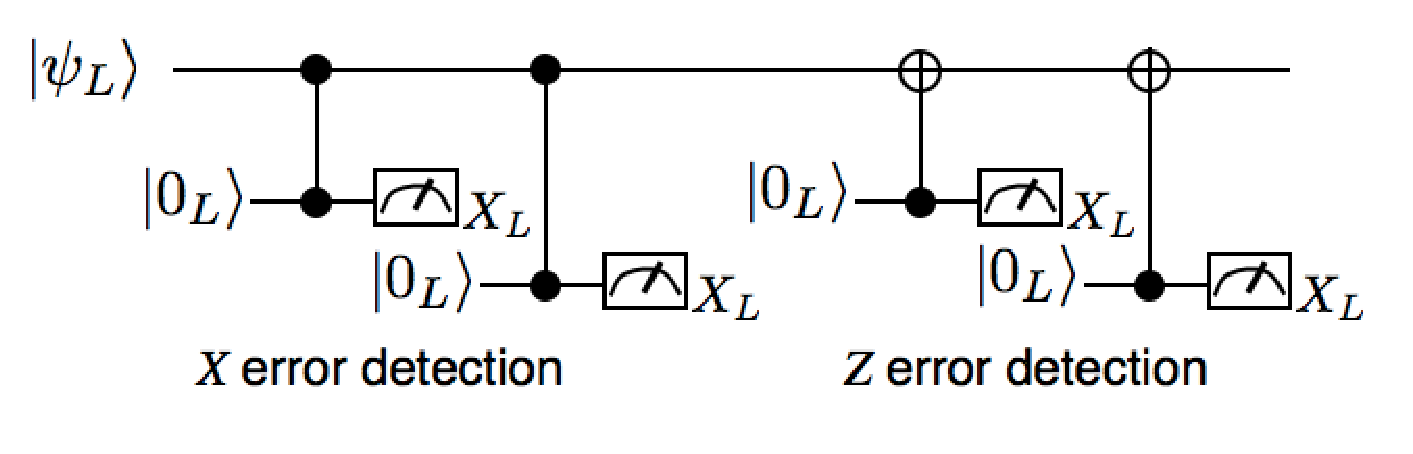
\includegraphics[width=100mm]{fig47.eps}
\end{equation}
%
Because the ancilla states are the logical code states, one can obtain the error syndrome by simply measuring the ancilla states.
The syndrome extraction is repeated a couple of times to extract reliable error information.
An optimized way to extract the syndrome information was proposed in Ref.~\cite{Plenio97}, where the subsequent syndrome extraction is performed conditionally according to the preceding syndrome information.
For these schemes to work fault-tolerantly, the encoded ancilla $|0_{L}\rangle$ states have to be prepared with high fidelity.
This is achieved by using either verification or entanglement purification \cite{KnillNature,Steane97,DAB03,ADB05}.


{\it Knill's gadget---}
Another interesting QEC gadget was proposed by Emanuel Knill \cite{KnillNature}.
It is based on quantum teleportation as illustrated in the following circuit:
%
\begin{equation}
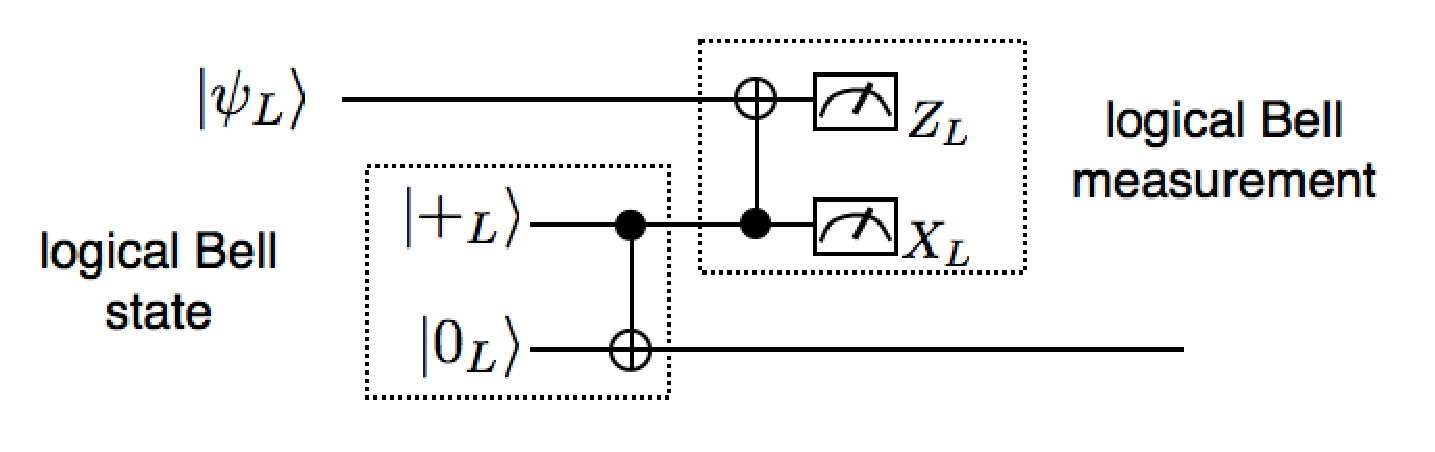
\includegraphics[width=100mm]{fig48.eps}
\end{equation}
%
Here, the encoded data qubit $|\psi _{L}\rangle$ is teleported to the fresh encoded qubit of the ancilla Bell state.
Thus, the encoded ancilla Bell state has to be prepared with high fidelity by using verification or entanglement purification, similarly to the Steane's gadget.
The logical Bell measurement completes the teleportation, namely {\it error-correcting teleportation}.
There is no need to identify the error syndrome, but 
it is sufficient to find the logical measurement outcomes of the logical Bell measurement.
Thus, it is not necessary to repeat the syndrome extraction in this QEC gadget.
The outcome of the Bell measurement is properly propagated to the subsequent computation as the Pauli frame \cite{KnillNature,Dawson06a,Dawson06b}.

\section{Fault-tolerant gate operations}
Fault-tolerant computation is now executed by the logical gate operations that are followed by the QEC gadgets.
This is illustrated for the fault-tolerant CNOT gate as follows:
%
\begin{equation}
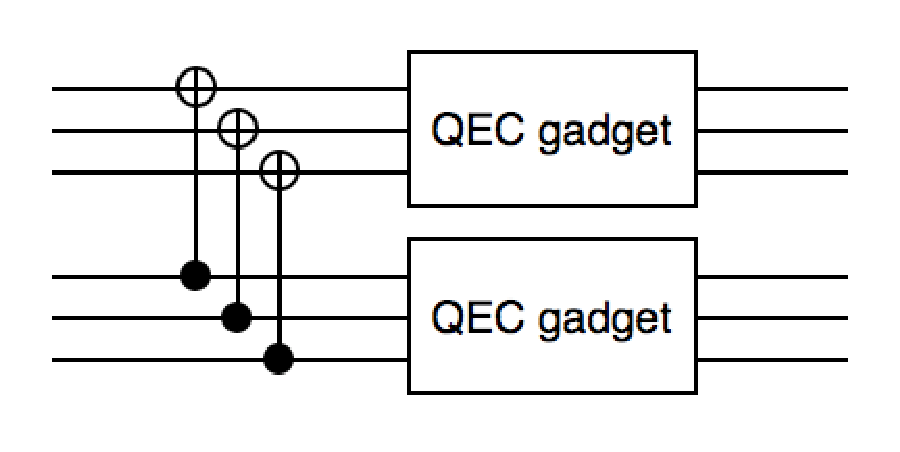
\includegraphics[width=70mm]{fig49.eps}
\label{fig:logicalgate}
\end{equation}
%
where the code block is depicted as though it is a three-qubit code.
A QEC gadget is attached to each logical output of the transversal CNOT gate.
Because a single error never will be propagated as multiple errors in a fault-tolerant gate, a logical error is caused by two (or more) simultaneous physical errors. 
Denoting the number of such faulty pairs of error locations as $C$, the logical error probability is given by $Cp^2$, with $p$ being the physical error probability.
If the physical error probability is sufficiently small, $p < 1/C$, one can improve the accuracy of the gate and achieve a fault-tolerant computation.

\section{Concatenated quantum computation}
For a reliable computation of a large size, the logical error probability should be reduced arbitrarily.
This is done by a concatenated fault-tolerant computation \cite{Knill98a,Knill98b,Aharonov97,Aharonov08}.
In the concatenated computation, each physical gate operation is repeatedly replaced by a logical gate operation followed by QEC gadgets.

Suppose $A$ is a quantum computation, which consists of some physical gate operations.
Then the first level concatenated computation is defined by $\mathcal{C} (A)$, where the operation $\mathcal{C}$ indicates replacing each physical gate with a logical one, followed by QEC gadgets. 
For example, $\mathcal{C}(\textrm{CNOT})$ is described in the diagram (\ref{fig:logicalgate}).
The second level concatenated CNOT gate $\mathcal{C} \circ \mathcal{C} (\textrm{CNOT})$ is also described as follows:
%
\begin{equation}
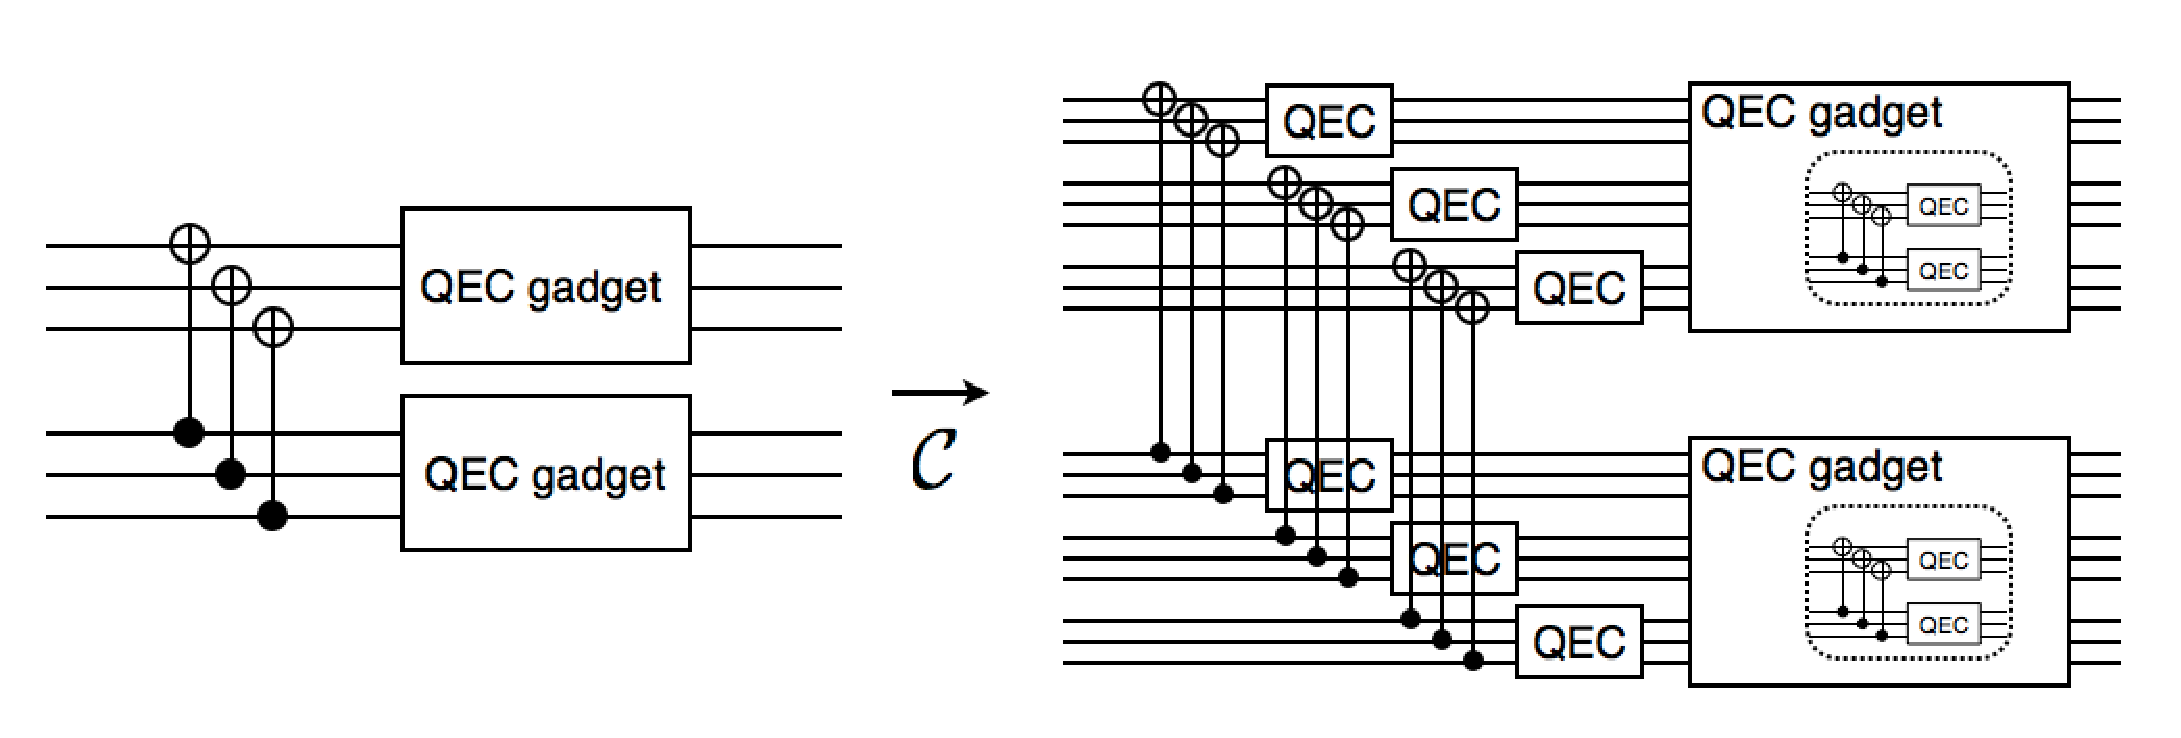
\includegraphics[width=130mm]{fig50.eps}
\label{fig:concatenated gate}
\end{equation}
%
where each physical gate in the QEC gadgets is replaced by the logical one, followed by the QEC gadgets.
By repeating this procedure, the $l$th level concatenated computation of $A$ is given by $\mathcal{C}^{l}(A)$.
Specifically, for a physical gate operation $G$ (e.g., Hadamard, CNOT gate, etc.), $\mathcal{C}^{l}(G)$ is called the level-$l$ $G$ gate.
The $l$th level concatenated code state is called the level-$l$ qubit, denoted by$|0^{(l)}\rangle$, $|+^{(l)}\rangle$.

As mentioned previously, the logical error probability $p_{g}^{(1)}$ of the level-1 gate is given by 
%
\begin{equation}
p^{(1)} = C (p^{(0)})^{2},
\end{equation}
%
where $p^{(0)}=p$ and $C$ denotes the number of all faulty pairs of error locations.
The constant $C$ differs between the logical gates.
It is, however, sufficient to choose the maximum value.
Due to the self-similarity of the concatenation, the logical error probability of the level-2 gate is given in terms of $p^{(1)}$ by 
%
\begin{equation}
p^{(2)} = C (p^{(1)})^{2}.
\end{equation}
%
Similarly, the logical error probability $p^{(l)}$ of the level-$l$ gate is obtained recursively as
%
\begin{eqnarray}
p^{(l)} &=& C (p^{(l-1)})^{2}
\nonumber \\
&=& (Cp^{(0)})^{2^{l}}/C.
\end{eqnarray}
%
We conclude that if $p^{(0)}<p_{\textrm{th}} \equiv 1/C$, the logical error probability can be reduced super-exponentially with the concatenation level $l$.
This is the so-called {\it threshold condition}.

On the other hand, the resources usage, $R^{(l)}$, consumed for the level-$l$ gate is estimated roughly as
%
\begin{equation}
R^{(l)}=N^{l},
\end{equation}
% 
where $N$ indicates the total number of physical gates in the level-1 gate.
Suppose that the size of the computation is $10^{n-1}=M$.
Then an accuracy of $p^{(l)} < 10^{-n}$ is required for each logical gate at the highest level. 
The total resources to perform a reliable quantum computation of size $M$ amount to 
%
\begin{eqnarray}
R_{\textrm{tot}}&=&N^{\bar{l}} M = \left( \frac{n}{\log _{10} (Cp^{(0)})^{-1}} \right)^{\log _{2} N}M = \textrm{poly}( \log (M))M,
\end{eqnarray}
%
where $\bar{l} \simeq \log _{2} \left[ n/\log _{10}(Cp^{(0)}) \right] $ is the number of levels necessary to achieve the required accuracy.
This result clearly shows that if the physical error probability $p^{(0)}$ is smaller than $p_{\textrm{th}}$, one can execute quantum computation to an arbitrary accuracy with only polylogarithmic overhead.
This is the celebrated {\it threshold theorem} and the critical value $p_{th}$ is called the {\it noise threshold} \cite{NielsenChuang,Kitaev97,Knill98a,Knill98b,Aharonov97}. 
%\subsection{How to estimate the noise thresholds}
The noise thresholds have been calculated to be about $10^{-4}-10^{-2}$ for several fault-tolerant schemes under varying degrees of assumption and rigor
\cite{Knill98a,Knill98b,Aharonov97,Aharonov08,Steane03,KnillNature,Aliferis06,Aliferis07,Aliferis08,Aliferis09,Steane99,Cross09}.
